
\newcommand{\jac}[2]{\frac{\partial #1}{\partial #2}}
\newcommand{\xhat}{\widehat{x}}
\newcommand{\yhat}{\widehat{y}}
\newcommand{\zhat}{\widehat{z}}
\newcommand{\vxhat}{\widehat\mathrm{x}}
\newcommand{\vzhat}{\widehat\mathrm{z}}
\newcommand{\setX}{\mathcal{X}}
\newcommand{\setB}{\mathcal{B}}
\newcommand{\E}{\text{E}}
\newcommand{\Var}{\text{Var}}
\newcommand{\Cov}{\text{Cov}}
\newcommand{\Fhat}{\widehat{F}}
\newcommand{\Thetahat}{\widehat{\Theta}}
\newcommand{\Norm}{\text{Norm}}
\newcommand{\BatchNorm}{\text{BN}}
\newcommand{\kk}{{(k)}}
\newcommand{\vx}{\mathrm{x}}
\newcommand{\vy}{\mathrm{y}}
\newcommand{\vp}{\mathrm{p}}
\newcommand{\vg}{\mathrm{g}}
\newcommand{\e}{\mathrm{E}}
\newcommand{\vu}{\mathrm{u}}
\newcommand{\mils}{\cdot 10^6}
\renewcommand{\algorithmicrequire}{\textbf{Input:}}
\renewcommand{\algorithmicensure}{\textbf{Output:}}
\newcommand{\rmax}{r_{\text{max}}}
\newcommand{\dmax}{d_{\text{max}}}


\begin{abstract}

批规范化可以十分有效地加速和提升深度模型的训练。但是,当训练的 minibatch 较小或不是由独立的样本组成时,它的有效性会降低。
我们假设这主要归因于如下两点,一是minibatch里样本的层输入之间有相关性,二是模型的训练和推理中输出的激活不同。
我们提出了一种简单有效的扩展——批再规范化,以确保训练和推理模型可以输出相同的激活,而且这个输出是基于单个样本而非整个 minibatch。
当训练时的minibatch比较小或者non-i.i.d.(非独立同分布)时,用批再规范化训练的模型表现显著优于批规范化训练的模型。
与此同时,批再规范化还保留了批规范化的优点,例如对初始化的不敏感和高训练效率。

Batch Normalization is quite effective at accelerating and improving the training of deep models. However, its effectiveness diminishes when the training minibatches are small, or do not consist of independent samples. We hypothesize that this is due to the dependence of model layer inputs on all the examples in the minibatch, and different activations being produced between training and inference. We propose Batch Renormalization, a simple and effective extension to ensure that the training and inference models generate the same outputs that depend on individual examples rather than the entire minibatch. Models trained with Batch Renormalization perform substantially better than batchnorm when training with small  or non-i.i.d. minibatches. At the same time, Batch Renormalization retains the benefits of batchnorm such as insensitivity to initialization and training efficiency.

\end{abstract}

\section{Introduction 简介}
批规范化近年来已经成为训练深度网络的标准工具包的一部分。通过规范化激活,批规范化使模型训练时内部激活的分布更加稳定,令训练时使用更高的学习率成为可能,并减少了模型对初始化的敏感度。这些影响可以增加训练速度,而且有时候甚至可以急剧增加训练速度。鉴于此,批规范化已经成功的应用于最先进的架构中,比如残差网络(residual networks)。

Batch Normalization (``batchnorm" \cite{batchnorm}) has recently become a part of the standard toolkit for training deep networks. By normalizing activations, batch normalization helps stabilize the distributions of internal activations as the model trains. Batch normalization also makes it possible to use significantly higher learning rates, and reduces the sensitivity to initialization. These effects help accelerate the training, sometimes dramatically so. Batchnorm has been successfully used to enable  state-of-the-art architectures such as residual networks \cite{resnet}.

批规范化对minibatch样本做随机梯度训练,并使用这些minibatch 样本的均值和方差去规范化激活。具体来说,考虑在深度网络中的一个特定节点,为每个输入样本产生一个标量值。给定$m$个样本的一个minibatch为$\setB$ ,考虑这个节点的值$x_1\ldots x_m$。 然后批规范化值如下所示:
$$
\xhat_i \leftarrow \frac{x_i-\mu_\setB}{\sigma_\setB}
$$

Batchnorm works on minibatches in stochastic gradient training, and uses the mean and variance of the minibatch  to normalize the activations. Specifically, consider a particular node in the deep network, producing a scalar value for each input example. Given a minibatch $\setB$ of $m$ examples, consider the values of this node, $x_1\ldots x_m$. Then batchnorm takes the form:
$$
\xhat_i \leftarrow \frac{x_i-\mu_\setB}{\sigma_\setB}
$$

这里的$\mu_\setB$ 是$x_1\ldots x_m$这m个样本的方差,$\sigma_\setB^2$ 是样本的方差(事实上,为了数值的稳定性增加了一个很小的值$\epsilon$)。
可以清楚的看到,对于输入一个样本的规范化激活将取决于minibatch中的其他样本,这在推断阶段是不可取的,因此可以用对整个训练样本计算均值和方差来代替只使用minibatch。
在实践中,模型经常会对minibatch的均值和方差计算移动平均,并在推断阶段使用这些移动平均来代替minibatch的统计量(均值,方差)。

where $\mu_\setB$ is the sample mean of $x_1\ldots x_m$, and $\sigma_\setB^2$ is the sample variance (in practice, a small $\epsilon$ is added to it for numerical stability). It is clear that the normalized activations corresponding to an input example will depend on the other examples in the  minibatch. This is undesirable during inference, and therefore the mean and variance computed over all training data can be used instead. In practice, the model usually maintains moving averages of minibatch means and variances, and during inference uses those in place of the minibatch statistics.

虽然批规范化似乎在推断阶段用整个数据取代了minibatch统计,改变了网络中的激活。事实上,这意味着以minibatch规范化作为输入的训练阶段跟以样本的统计规范化作为输入的推断阶段是不同的。当minibatch 比较大或者训练样本的分布是独立同分布的时候,这种差异是很小的,所以有利于泛化,但是,minibatch范围内的规范化有一些显著的缺点。

While it appears to make sense to replace the minibatch statistics with whole-data ones during inference, this changes the activations in the network. In particular, this means that the upper layers (whose inputs are normalized using the minibatch) are trained on representations different from those computed in inference (when the inputs are normalized using the population statistics). When the minibatch size is large and its elements are i.i.d. samples from the training distribution, this difference is small, and can in fact aid generalization. However,  minibatch-wise normalization may have significant drawbacks:

对于比较小的minibatch,均值和方差的估计变得不太精确。这些不确定性再加上深度,会降低最终模型结果的准确度。而且,由于在规范化中使用的方差,是用这些被规范的样本本身来计算的,所以这些规范化参数的估计不是很好。而这些参数将会被用于推算阶段的计算中。(译者注:每个小批量用自己来规范自己,这种做法在小批量本身对全体训练样本不具有足够的代表性的时候,会产生偏差)
For {\em small minibatches}, the estimates of the mean and variance become less accurate. These inaccuracies are compounded with depth, and reduce the quality of resulting models. Moreover, as each example is used to compute the variance used in its own normalization, the normalization operation is less well approximated by an affine transform, which is what is used in inference.

{\em 非独立同分布minibatch }可能对模型的规范化产生不利影响。例如,在度量学习的场景中,经常会偏差化minibatch样本包括显著相关的样本集。
例如,对于一个大小为32的minibatch,我们可能随机选择16个标签,然后从每个标签中选出两个样本。
没有规范化的话,对于minibatch 的损失计算与整个样本解耦,在我们的采样机制中引入的批内依赖,在最差的情况下,会增加训练时minibatch梯度的方差。
有了规范化的话,这些样本与每一层都相互作用,从而可能导致模型为了适应那些特别的minibatch分布而产生过拟合,但是对于个别样本表现糟糕。

{\em Non-i.i.d. minibatches} can have a detrimental effect on models with batchnorm. For example, in a metric learning scenario (e.g. \cite{nca}), it is common to bias the minibatch sampling to include sets of examples that are known to be related. For instance, for a minibatch of size 32, we may randomly select 16 labels, then choose 2 examples for each of those labels. Without batchnorm, the loss computed for the minibatch decouples over the examples, and the intra-batch dependence introduced by our sampling mechanism may, at worst, increase the variance of the minibatch gradient. With batchnorm, however, the examples interact at every layer, which may cause the model to overfit to the specific distribution of minibatches and suffer when used on individual examples.

依赖于整个minibatch批规范化激活使批规范化更有效,但是这也是它的缺陷来源。已经提出几种方法来减弱它的缺点\cite{weightnorm,layernorm,normprop}。但是,不像批规范化那样易于被应用在网络中,那些方法可能要求仔细的非线性分析与minibatch 中心结合,可能改变模型的函数表示类别。另一个方法是\cite{gan},使用一个独立固定的minibatch来计算规范化参数,但是,它使训练代价更大。

The dependence of the batch-normalized activations on the entire minibatch makes batchnorm powerful, but it is also the source of its drawbacks. Several approaches \cite{weightnorm,layernorm,normprop} have been proposed to alleviate this. However, unlike batchnorm which can be easily applied to a network, these methods may require careful analysis of nonlinearities, may need to be combined with  minibatch centering, and may change the class of functions representable by the model. Another alternative \cite{gan} is to use a separate and fixed minibatch to compute the normalization parameters, but this makes the training more expensive.

本文中,我们提出批再规范化,对于批规范化的一种新扩展。我们的方法保证与推断过程的激活计算一样,在训练步骤的前趟激活计算只依赖于单个样本。这明显的改善了小minibatch和非独立同分布的训练,跟批规范化相比,没有额外的开销。

In this paper we propose {\em Batch Renormalization}, a new extension to batchnorm. Our method ensures that the activations computed in the forward pass of the training step depend only on a single example and are identical to the activations computed in inference. This significantly improves the training on non-i.i.d. or small minibatches, compared to batchnorm, without incurring extra cost.

\section{Prior Work: Batch Normalization先前工作:批规范化}
我们的研究兴趣在于深度网络的随机梯度优化,目标是最小化类似如下这种由整个训练集共同定义的损失函数。
$$\Theta = \arg \min_\Theta
\frac{1}{N}\sum_{i=1}^N \ell_i(\Theta)$$

We are interested in stochastic gradient optimization of deep networks. The task is to minimize the loss, which decomposes over training examples:
$$\Theta = \arg \min_\Theta
\frac{1}{N}\sum_{i=1}^N \ell_i(\Theta)$$

这里$\ell_i$ 是训练样本的损失,$\Theta$是模型权重向量。在每个训练步骤,$m$ 个训练样本的一个minibatch被用来计算梯度$$\frac{1}{m} \jac{ \ell_i(\Theta)}{ \Theta}$$,对梯度的优化来调整$\Theta$。
where $\ell_i$ is the loss incurred on the $i$th training example, and $\Theta$ is the vector of model weights. At each training step, a minibatch of $m$ examples is used to compute the  gradient
$$\frac{1}{m} \jac{ \ell_i(\Theta)}{ \Theta}$$
which the optimizer uses to adjust $\Theta$.

考虑深度网络中的一个特定节点$x$。我们注意到计算$x$依赖所有模型参数,模型参数一改变,$x$的分布也会改变。由于它自己影响所有在它之上的层的损失函数,这种分布的改变会导致训练复杂化,这被称为内部协变量转移。

Consider a particular node $x$ in a deep network. We observe that $x$ depends on all the model parameters that are used for its computation, and when those change, the distribution of $x$ also changes. Since $x$ itself affects the loss through all the layers above it, this change in distribution complicates the training of the layers above. This has been referred to as internal covariate shift.

批规范化通过调整一个minibatch $\setB=\{x_{1\ldots m}\}$ 的激活输出$x$来解决这个问题。用以下公式规范化$x$:
Batch Normalization \cite{batchnorm} addresses it by considering the values of $x$ in a minibatch $\setB=\{x_{1\ldots m}\}$. It then normalizes them as follows:
\begin{align*}
    \mu_\setB &\leftarrow \frac{1}{m}\sum_{i=1}^m x_i\\
  \sigma_\setB &\leftarrow  \sqrt{\frac{1}{m}\sum_{i=1}^m (x_i-\mu_\setB)^2+\epsilon}\\
\xhat_i &\leftarrow \frac{x_i-\mu_\setB}{\sigma_\setB}
\\
  y_i &\leftarrow \gamma\xhat_i + \beta  \equiv \BatchNorm(x_i)
\end{align*}

这里的$\gamma$ 和 $\beta$ 是训练参数(在同一过程中学习,例如随机梯度下降,跟所有其他的模型权重一样),$\epsilon$ 是一个很小的常数。最重要的是,样本均值 $\mu_\setB$和样本标准差$\sigma_\setB$的计算是模型结构的一部分,它们作为模型参数的函数参与反向传播。对于batchnorm传播公式可以使用简单的链式法则来得出,具体计算可参考\cite{batchnorm}。

Here $\gamma$ and $\beta$ are trainable parameters (learned using the same procedure, such as stochastic gradient descent, as all the other model weights), and $\epsilon$ is a small constant. Crucially, the computation of the sample mean $\mu_\setB$ and sample standard deviation $\sigma_\setB$ are part of the model architecture, are themselves functions of the model parameters, and as such participate in backpropagation. The backpropagation formulas for batchnorm are easy to derive by chain rule and are given in \cite{batchnorm}.

当在一个激活层$\vx$上使用批规范化时,我们单独规范化激活的各个维度(或者,卷积网络中的每个通道特征映射)

When applying batchnorm to a layer of activations $\vx$, the normalization takes place independently for each dimension (or, in the convolutional case, for each channel or feature map).

当$\vx$自己是对前一层的线性变化时,批规范化使模型优化过程不受$W$中参数绝对值大小的影响(忽略小$\epsilon$),这种不变性使模型训练不依赖于初始化,并令使用更大的学习率成为可能。

When $\vx$ is itself a result of applying a linear transform $W$ to the previous layer, batchnorm makes the model invariant to the scale of $W$ (ignoring the small $\epsilon$). This invariance makes it possible to not be picky about weight initialization, and to use larger learning rates.

除了减少内部变量转变之外,批规范化的另一个作用,可以通过考察梯度在不同层间的传播来得到一个直观的认识。考虑一个特殊的例子,假设规范化层$\vxhat$中元素均具有零均值和单位方差。我们来做一个思想实验,让我们假设$\vxhat$ 的各个维度之间是独立的高斯分布,而且,假设损失函数$\ell$有一个线性近似$\vxhat$: $\ell = \vg^T \vxhat$,其中$\vg = \jac{\ell}{\vxhat}$.那么$\|\vg\|^2 = \Var[\ell]$ 只取决于模型的损失函数,而不取决于我们选择的层。这意味着梯度范数$\|\jac{\ell}{\vxhat}\|$在任何一个规范化的层上都是一样的。
因此,在梯度流经整个网络的过程中,不会发生梯度爆炸也不会发生梯度消失,从而促进训练效率。虽然独立性假设,高斯假设和以及线性假设在实践中都不成立,但是批规范化还是明显的改善了梯度流。

Besides the reduction of internal covariate shift, an intuition for another effect of batchnorm can be obtained by looking at the gradients computed by backpropagation for different layers. Consider the normalized layer $\vxhat$, whose elements all have zero mean and unit variance. For a thought experiment, let us assume that the dimensions of $\vxhat$ are  Gaussian and independent. Further, let us approximate the loss $\ell$ as a linear function of $\vxhat$: $\ell = \vg^T \vxhat$, where $\vg = \jac{\ell}{\vxhat}$. It then follows that  $\|\vg\|^2 = \Var[\ell]$ which only depends on the model loss and not the layer we picked. This means that the norm of the gradient w.r.t. a normalized layer $\|\jac{\ell}{\vxhat}\|$ is the same for different normalized layers. Therefore the gradients, as they flow through the network, do not explode nor vanish, thus facilitating the training. While the assumptions of independence, Gaussianity and linearity do not hold in practice, the gradient flow is in fact significantly improved in batch-normalized models.

在推断阶段,标准的做法是使用移动平均 $\mu$, $\sigma^2$ 而不是minibatch的均值$\mu_\setB$方差$\sigma_\setB^2$来规范化激活。这使得如下的规范化激活仅取决于单个输入样本,而不是整个minibatch.
$$
y_\text{inference} = \frac{x-\mu}{\sigma}\cdot \gamma + \beta
$$

During inference, the standard practice is to normalize the activations using the moving averages $\mu$, $\sigma^2$ instead of minibatch mean $\mu_\setB$ and variance $\sigma_\setB^2$:
$$
y_\text{inference} = \frac{x-\mu}{\sigma}\cdot \gamma + \beta
$$
which depends only on a single input example rather than requiring a whole minibatch.

一个很自然的问题是,我们是否可以简单的在训练过程中使用移动平均$\mu$, $\sigma$来进行规范化,因为这样做可以取消minibatch中样本的内部相关性。然而,我们已经注意到这样会导致模型发散。正如批规范\cite{batchnorm}中讨论的一样,使用移动平均将导致梯度优化与规范化相互抵消。例如,梯度步骤可能增加一个偏差或者缩放的卷积权重,尽管事实上规范化将消除这些变化对损失的影响。这将导致无限增长的模型参数,而实际上却不改变损失函数。因此,至关重要的是使用minibatch的动量并通过他们反向传播。

It is natural to ask whether we could simply use the moving averages $\mu$, $\sigma$ to perform the normalization during training, since this would remove the dependence of the normalized activations on the other example in the minibatch. This, however, has been observed to lead to the model blowing up. As argued in \cite{batchnorm}, such use of moving averages would cause the gradient optimization and the normalization to counteract each other. For example, the gradient step may increase a bias or scale the convolutional weights, in spite of the fact that the normalization would cancel the effect of these changes on the loss. This would result in unbounded growth of model parameters without actually improving the loss. It is thus crucial to use the minibatch moments, and to backpropagate through them.

\section{Batch Renormalization批再规范化}
批规范化时,由于规范化的不同,网络在训练和推断过程中会输出不同的激活。本文主要目的是在保留批规范化的优点的同时改善这一情况。

With batchnorm, the activities in the network differ between training and inference, since the normalization is done differently between the two models. Here, we aim to rectify this, while retaining  the benefits of batchnorm.

如果我们有一个minibatch,可以使用minibatch自己的统计值或者他们统计值的移动平均来规范化一个节点$x$,这两种规范化结果之间是一个仿射变换的关系。
$$
\frac{x_i-\mu}{\sigma} = \frac{x_i-\mu_\setB}{\sigma_\setB} \cdot r + d,\ \ \ \ \text{where $ r = \frac{\sigma_\setB}{\sigma}, \ \  d = \frac{\mu_\setB-\mu}{\sigma}$}
$$

Let us observe that if we have a minibatch and normalize a particular node  $x$ using either the minibatch statistics or their moving averages, then the results of these two normalizations are related by an affine transform.

特别的,令$\mu$是$x$的一个均值的估计,$\sigma$是标准差的估计值(可以通过最后几个minibatch的移动平均来实现),那么:

Specifically, let $\mu$ be an estimate of the mean of $x$, and $\sigma$ be an estimate of its standard deviation, computed perhaps as a moving average over the last several minibatches. Then, we have:
$$
\frac{x_i-\mu}{\sigma} = \frac{x_i-\mu_\setB}{\sigma_\setB} \cdot r + d,\ \ \ \ \text{where $ r = \frac{\sigma_\setB}{\sigma}, \ \  d = \frac{\mu_\setB-\mu}{\sigma}$}
$$

如果$\sigma = \e[\sigma_\setB]$,$\mu=\e[\mu_\setB]$,那么 $\e[r] = 1$,$\e[d] = 0$(对于minibatch$\setB$计算期望)。事实上,批规范化等同简单的预设了$r=1$, $d=0$.

If  $\sigma = \e[\sigma_\setB]$ and $\mu=\e[\mu_\setB]$, then $\e[r] = 1$ and $\e[d] = 0$  (the expectations are w.r.t. a minibatch $\setB$). Batch Normalization, in fact, simply sets $r=1$, $d=0$.

我们建议保留$r$和$d$,但是在计算梯度时把他们作为常数处理。
换句话说,我们在一个含有批规范化层的网络中对于每一个规范化的激活函数进行了一个一维的仿射变换。
我们把$r$ 和$d$当成固定的常数,即便他们是从minibatch本身计算出来的。
值得注意的是,只要$\sigma = \e[\sigma_\setB]$,$\mu=\e[\mu_\setB]$,那么这个变换的期望实际上是恒同变换。
我们提出使用这种仿射变换的批规范化作为{\em 批再规范化}:对于指定的minibatch,$r$ 和$d$对minibatch本身的统计值进行修正。
它将允许上层观察到这个相对"正确"的激活值,即,将来被推断模型产生的那个激活值。

We propose to retain $r$ and $d$, but treat them as constants for the purposes of gradient computation. In other words, we augment a  network, which contains batch normalization layers, with a per-dimension affine transformation applied to the normalized activations. We treat the parameters $r$ and $d$ of this affine transform as fixed, even though they were computed from the minibatch itself. It is important to note that this transform  is identity in expectation, as long as  $\sigma = \e[\sigma_\setB]$ and $\mu=\e[\mu_\setB]$. We refer to batch normalization augmented with this affine transform as {\em Batch Renormalization}: the fixed (for the given minibatch) $r$ and $d$ correct for the fact that the minibatch statistics differ from the population ones. This allows the above layers to observe the ``correct"  activations -- namely, the ones that would be generated by the inference model.

实际上,一个比较好的做法是现用批规范化进行若干次迭代,然后再引入批再规范化。我们的做法是先分别限制$r=1$和$d=0$,然后再把这个限制慢慢放宽。

In practice, it is beneficial to train the model for a certain number of iterations with batchnorm alone, without the correction, then ramp up the amount of allowed correction. We do this by imposing bounds on $r$ and $d$, which initially constrain them to $1$ and $0$, respectively, and then are gradually relaxed.

\begin{algorithm}[t]
  \caption{\em 使用批再规范化的训练(上)和推理(下),其在一个 minibatch 上应用了激活 x。在反向传播过程中使用了标准的链式法则。用 stop-gradient 标记的值被当作一个给定训练步骤的常量处理,而且该梯度不会经由它们传播。
  }
  \caption{\em Training (top) and inference (bottom) with Batch Renormalization, applied to activation $x$ over a mini-batch. During backpropagation, standard chain rule is used.
  The values marked with \texttt{stop\_gradient} are treated as constant for a given training step, and the gradient is not propagated through them.
  }
\label{alg-bn}
  \begin{algorithmic}
  \REQUIRE
  对于一个训练mini-batch,$x$的值
  Values of $x$ over a training mini-batch
  $\setB=\{x_{1\ldots m}\}$;
  参数$\gamma$,

 parameters $\gamma$,$\beta$; 目前的均值 $\mu$ ,标准差 $\sigma$; 移动平均更新率$\Delta$; 最大被允许修正值 $\rmax$, $\dmax$.
    $\beta$; current moving mean $\mu$ and standard deviation $\sigma$; moving average update rate $\Delta$; maximum allowed correction $\rmax$, $\dmax$.
  \ENSURE $\{y_i =  \text{BatchRenorm}(x_i)\}$; updated $\mu$, $\sigma$.
  \begin{flalign*}
      \mu_\setB &\leftarrow  \frac{1}{m}\sum_{i=1}^m x_i \\
  \sigma_\setB &\leftarrow  \sqrt{\epsilon + \frac{1}{m}\sum_{i=1}^m (x_i-\mu_\setB)^2 }
\\
  r &\leftarrow \mathtt{stop\_gradient}\left(\text{clip}_{[1/\rmax, \rmax]}\left( \frac{\sigma_\setB}{\sigma}\right)\right) \\
  d &\leftarrow  \mathtt{stop\_gradient}\left(\text{clip}_{[-\dmax, \dmax]}\left(\frac{\mu_\setB-\mu}{\sigma}\right)\right)
  \\
\xhat_i &\leftarrow \frac{x_i-\mu_\setB}{\sigma_\setB} \cdot r + d
\\
  y_i &\leftarrow \gamma\,\xhat_i + \beta   \\
  \\
  \mu & \mathrel{:}= \mu + \Delta (\mu_\setB - \mu) \hspace{0.2in} \text{ // Update moving averages}\\
  \sigma &\mathrel{:}=  \sigma + \Delta (\sigma_\setB - \sigma)
  \end{flalign*}
  \hspace{-.1in}\hrulefill\hspace{.03in}\\
  \vspace{-0.1in}
    \hspace{-.1in}\hrulefill\hspace{.03in}\\
  \vspace{.2in}
  \item[\textbf{Inference:}]\ \ \ \ \ \ \
  $\displaystyle y\leftarrow \gamma\cdot \frac{x-\mu}{\sigma} + \beta$
    \vspace{.1in}
\end{algorithmic}
\end{algorithm}

算法\ref{alg-bn} 呈现了批再规范化。不像批规范化,训练的移动平均只在推断中使用,批再规范化使用$\mu$ 和$\sigma$在训练中用来执行纠正。我们对这些平均值采用比较高的更新率$\Delta$,以确保这些平均值既可以吸收多个minibatch的平均值,有可以具有跟模型参数相当的更新率。我们用指数衰减来更新移动平均$\mu$ 和 $\sigma$,并使用反向传播的梯度计算方法来优化模型的其余部分。

Algorithm \ref{alg-bn} presents Batch Renormalization. Unlike batchnorm, where the moving averages are computed during training but used only for inference, Batch Renorm does use $\mu$ and $\sigma$ during training to perform the correction. We use a fairly high rate of update $\Delta$ for these averages, to ensure that they benefit from averaging multiple batches but do not become stale relative to the model parameters. We explicitly update the exponentially-decayed moving averages $\mu$ and $\sigma$, and optimize the rest of the model using gradient optimization, with the gradients calculated via backpropagation:

\begin{align*}
\jac{\ell}{\xhat_i} &= \jac{\ell}{y_i}\cdot \gamma \\
\jac{\ell}{\sigma_\setB}
&= \sum_{i=1}^m \jac{\ell}{\xhat_i}\cdot(x_i-\mu_\setB)\cdot
\frac{-r}{\sigma_\setB^2} \\
\jac{\ell}{\mu_\setB} &=
\sum_{i=1}^m \jac{\ell}{\xhat_i}\cdot
\frac{-r}{\sigma_\setB}\\
   \jac{\ell}{x_i} &= \jac{\ell}{\xhat_i} \cdot
\frac{r}{\sigma_\setB} + \jac{\ell}{\sigma_\setB}\cdot
\frac{x_i-\mu_\setB}{m \sigma_\setB} + \jac{\ell}{\mu_\setB}\cdot \frac{1}{m}\\
\jac{\ell}{\gamma}&= \sum_{i=1}^m \jac{\ell}{y_i} \cdot \xhat_i
  \\
  \jac{\ell}{\beta} &= \sum_{i=1}^m \jac{\ell}{y_i}
\end{align*}

这些梯度方程揭露了批再规范化的另一种解释,因为当$x_i$平移或者缩放相同倍数时,损失$\ell$是不受影响的
These gradient equations reveal another interpretation of Batch Renormalization. Because the loss $\ell$ is unaffected when all $x_i$ are shifted or scaled by the same amount,

函数$\ell(\{x_i+t\})$和$\ell(\{x_i\cdot(1+t)\})$关于$t$中是常数,在$t=0$计算他们的导数,给出
$\sum_{i=1}^m \jac{\ell}{x_i} = 0$ 和 $\sum_{i=1}^m x_i\,\jac{\ell}{x_i} = 0$.因此,如果我们考虑$m$维向量$\big\{\jac{\ell}{x_i}\big\}$(在这个minibatch的每个样本的每个元素),进而考虑两个向量$\vp_0=(1,\ldots,1)$ 和 $\vp_1=(x_1,\ldots,x_m)$,所以$\big\{\jac{\ell}{x_i}\big\}$包含在$\vp_0$ 和 $\vp_1$的零空间中。

the functions $\ell(\{x_i+t\})$ and $\ell(\{x_i\cdot(1+t)\})$ are constant in $t$, and computing their derivatives at $t=0$ gives $\sum_{i=1}^m \jac{\ell}{x_i} = 0$ and $\sum_{i=1}^m x_i\,\jac{\ell}{x_i} = 0$. Therefore, if we consider the $m$-dimensional vector $\big\{\jac{\ell}{x_i}\big\}$ (with one element per example in the minibatch), and further consider two vectors
$\vp_0=(1,\ldots,1)$ and $\vp_1=(x_1,\ldots,x_m)$, then $\big\{\jac{\ell}{x_i}\big\}$ lies in the null-space of $\vp_0$ and $\vp_1$.

事实上,很容易在批再规范化的反向传播函数中看出,为了从$\big\{\jac{\ell}{x_i}\big\}$中计算梯度$\big\{\jac{\ell}{\xhat_i}\big\}$,我们需要首先用$r/\sigma_\setB$对前者进行调整,然后将其投影到$\vp_0$ 和 $\vp_1$的零空间,这个相当于对变换$\frac{x-\mu}{\sigma}$进行结合了零空间投影的反向传播。换言之,批再规范化利用在反向传播中加入额外投影层的办法,来达到允许我们在训练中使用移动平均$\mu$和$\sigma$来进行规范化的目的。

In fact, it is easy to see from the Batch Renorm backprop formulas that to compute the gradient $\big\{\jac{\ell}{x_i}\big\}$ from  $\big\{\jac{\ell}{\xhat_i}\big\}$, we need to first scale the latter by $r/\sigma_\setB$, then project it onto the null-space of $\vp_0$ and $\vp_1$. For $r=\frac{\sigma_\setB}{\sigma}$, this is equivalent to the backprop for the transformation $\frac{x-\mu}{\sigma}$, but combined with the null-space projection. In other words, Batch Renormalization allows us to normalize using moving averages $\mu$, $\sigma$ in training, and makes it work using the extra projection step in backprop.

批再规范化跟批规范化有许多有益的共同点,比如对初始化不敏感和以更高的学习率进行有效的训练。但是比批规范化好的地方在于,批再规范化保证模型训练时每一层的内部表示与推断时的内部表示是一致的。

Batch Renormalization shares many of the beneficial properties of batchnorm, such as insensitivity to initialization and ability to train efficiently with large learning rates. Unlike batchnorm, our method ensures that that all layers are trained on internal representations that will be actually used during inference.

\section{Results}
为了评估批再规范化,我们把它应用到图像分类的问题。我们的基线模型是inception-v3模型训练1000个类的ImageNet训练集,并在ImageNet 数据进行验证。在基线模型,批规范化在卷积之后,ReLU 之前。
To evaluate Batch Renormalization, we applied it to the problem of image classification. Our baseline model is Inception v3 \cite{inception-v3}, trained on 1000 classes from ImageNet training set \cite{imagenet}, and evaluated on the ImageNet validation data. In the baseline model, batchnorm was used after convolution and before the ReLU \cite{relu}.

应用批再规范化,我们只是简单的在模型中让它代替批规范化。这两种方法规范每个特征映射到样本以及样本的空间位置。我们固定大小$\gamma=1$,因为它可以通过ReLU传播吸收进入下一层。
To apply Batch Renorm, we simply swapped it into the model in place of batchnorm. Both methods normalize each feature map over examples as well as over spatial locations. We fix the scale $\gamma=1$, since it could be propagated through the ReLU and absorbed into the next layer.

训练使用50个同步的worker,每个worker每一个训练步骤处理一个32个样本的minibatch。所有50个minibatch 的梯度计算进行汇总,然后使用RMSProp优化器。通常的做法是,推断模型使用所有模型参数的指数衰减移动平均,包括批规范化和批再规范化都要计算的$\mu$ 和 $\sigma$。
The training used 50 synchronized workers \cite{syncreplicas}. Each worker processed a minibatch of 32 examples per training step. The gradients computed for all 50 minibatches were aggregated and then used by the RMSProp optimizer \cite{rmsprop}. As is common practice, the inference model used exponentially-decayed moving averages of all model parameters, including the $\mu$ and $\sigma$ computed by both batchnorm and Batch Renorm.

对批再规范化,开始的5000个训练步骤,我们使用$\rmax=1$, $\dmax=0$(就是简单的批规范化),之后逐渐放松,直到在40k步时达到$\rmax=3$,在25k步时$\dmax=5$ 
For Batch Renorm, we used $\rmax=1$, $\dmax=0$ (i.e. simply batchnorm) for the first 5000 training steps, after which these were gradually relaxed to reach $\rmax=3$ at 40k steps, and $\dmax=5$ at 25k steps. These final values resulted in clipping a small fraction of $r$s, and none of $d$s. However, at the beginning of training, when the learning rate was larger, it proved important to increase $\rmax$ slowly: otherwise, large gradients were observed to suddenly and severely increase the loss. We have found clipping to be less important for those Batch Renorm layers that are followed by another normalization layer. The intuition is that for such layers, scaling up all the corrections $r$ will leave the model output and gradients unchanged since the next normalization layer will cancel out the effects the larger correction.

除了与规范化有关的参数,所有超参数的值在模型和整个实验中是固定的。
All the hyperparameters other than those related to normalization were fixed between the models and across experiments.

\subsection{Baseline}

\begin{figure}
    \centering
    \begin{tabular}{@{}c@{}}
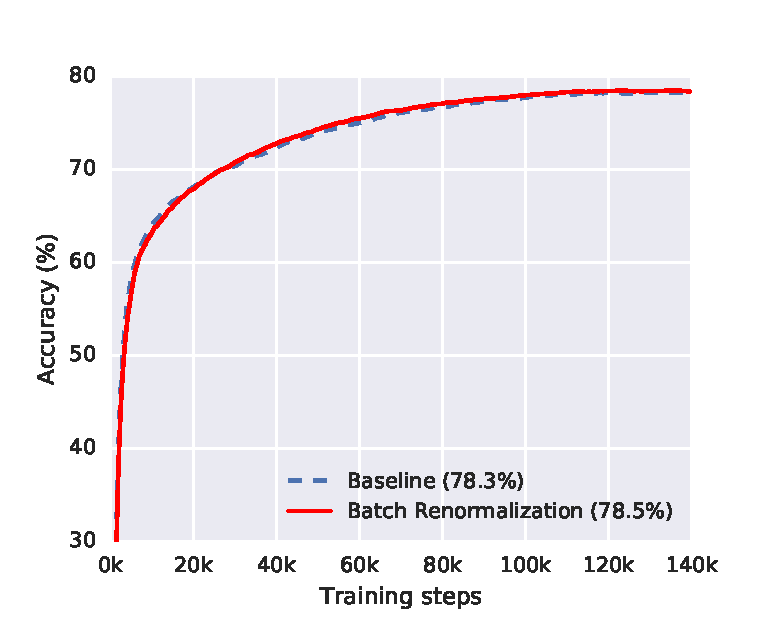
\includegraphics[width=\columnwidth]{baseline.eps}
\end{tabular}
    \caption{\em 分别使用批规范化和批再规范化的 Inception-v3 模型的验证 top-1 准确度(validation top-1 accuracy),模型是在 50 个同步的工作器(worker)上训练的,其中每一个工作器处理大小为 32 的 minibatch。使用批再规范化的模型实现了略高一点的验证准确度。
    }
    \caption{\em Validation top-1 accuracy of Inception-v3 model with batchnorm and its Batch Renorm version, trained on 50 synchronized workers, each processing minibatches of size 32. The Batch Renorm model achieves a marginally higher validation accuracy.
    }
    \label{fig-baseline}
\end{figure}

作为基线,我们使用大小为32的minibatch批规范化模型训练,更特定的,批规范化被应用在50个minibatch的每一个;每个样本使用32个样本规范化,但是梯度计算的结果在50个minibatch上汇总,这个模型验证 top-1 准确度在130k 训练步后为$78.3\%$
As a baseline, we trained the batchnorm model using the minibatch size of 32. More specifically, batchnorm was applied to each of the 50 minibatches; each example was normalized using 32 examples, but the resulting gradients were aggregated over 50 minibatches. This model achieved the top-1 validation accuracy of $78.3\%$ after 130k training steps.

为了验证批再规范化并没有在这样的minibatch上减少性能,我们也训练批规范化模型,见表\ref{fig-baseline}。模型的测试结果接近基线,在同样步后取得了稍微更高的测试准确度($78.5\%$)。
To verify that Batch Renorm does not diminish performance on such minibatches, we also trained the model with Batch Renorm, see Figure \ref{fig-baseline}. The test accuracy of this model closely tracked the baseline, achieving a slightly higher test accuracy ($78.5\%$) after the same number of steps.

\subsection{Small minibatches}
\begin{figure}
    \centering
    \begin{tabular}{@{}c@{}}
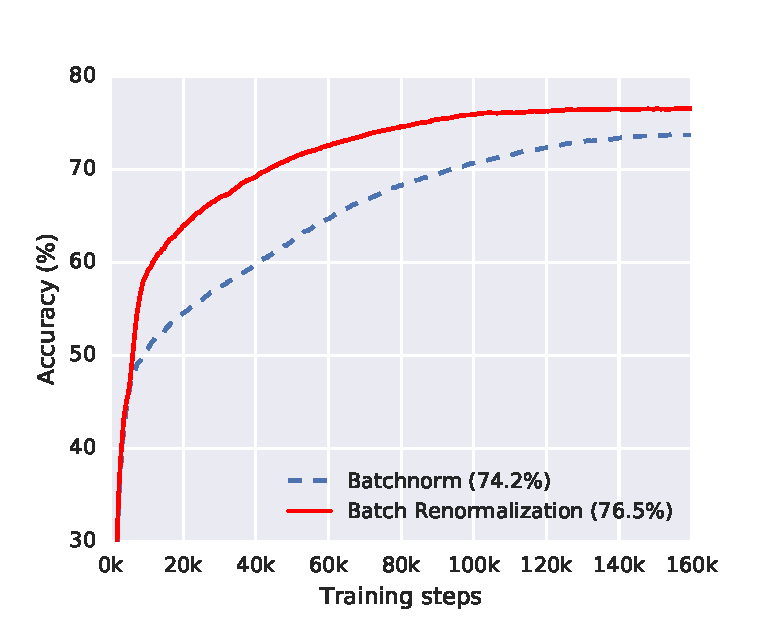
\includegraphics[width=\columnwidth]{small.eps}
\end{tabular}
    分别使用批规范化和批再规范化的模型的验证准确度,其中规范化是在有 4 个样本的集合上执行的(但带有被 50 个工作器处理过的在所有 50×32 个样本上聚集的梯度)。批再规范化让模型能更快地训练和实现更高的准确度,尽管规范化 32 个样本的集合会表现更好。
    \caption{\em Validation accuracy for models trained with either batchnorm or Batch Renorm, where normalization is performed for sets of 4 examples (but with the gradients aggregated over all $50\times 32$ examples processed by the 50 workers). Batch Renorm allows the model to train faster and achieve a higher accuracy, although normalizing sets of 32 examples performs better.
    }
    \label{fig-small}
\end{figure}
为了探索批再规范化在小minibatch训练的有效性,我们减少使用规范化的样本的数量到4.每个大小为32的minibatch因此被分为只有4个样本的更小的microbatches;每个microbatches被单独规范化,但是,每个minibatch的损失仍按照之前那样计算。换句话说,每个步骤的梯度仍然是汇总1600个样本,但是规范化只涉及4个样本的组合而不是基线中的32个样本,表\ref{fig-small}呈现了结果。
To investigate the effectiveness of Batch Renorm when training on small minibatches, we reduced the number of examples  used for normalization to 4. Each minibatch of size 32 was thus broken into ``microbatches" each having 4 examples; each microbatch was normalized independently, but the loss for each minibatch was computed as before. In other words, the gradient was still aggregated over 1600 examples per step, but the normalization involved groups of 4 examples rather than 32 as in the baseline. Figure \ref{fig-small} shows the results.

这种验证中,批规范化模型的精度明显更低于基线中minibatch大小为32的规范化,并且训练速度慢,在210k步后得到$74.2\%$。我们通过把批规范化替换为批再规范化后,得到一个速度更快的实质性的改善(在130k steps 后130k steps),但是测试精度仍然低于大小为32的minibatch的批规范化和批再规范化。虽然批再规范化改善了小minibatch训练,不排除它有更大的收益。
The validation accuracy of the batchnorm model is significantly lower than the baseline that normalized over minibatches of size 32, and training is slow, achieving $74.2\%$ at 210k steps. We obtain a substantial improvement much faster (130k steps at 130k steps) by replacing batchnorm with Batch Renorm, However, the resulting test accuracy is still below what we get when applying either batchnorm or Batch Renorm to size 32 minibatches. Although Batch Renorm improves the training with small minibatches, it does not eliminate the benefit of having larger ones.


% We observed a further increase in validation accuracy to $76.8\%$ when the maximum correction ratio $\rmax$ is further increased for those Batch Renorm layers that are followed by another normalization layer.


\subsection{Non-i.i.d. minibatches}
\begin{figure}[t]
    \centering
    \begin{tabular}{@{}c@{}}
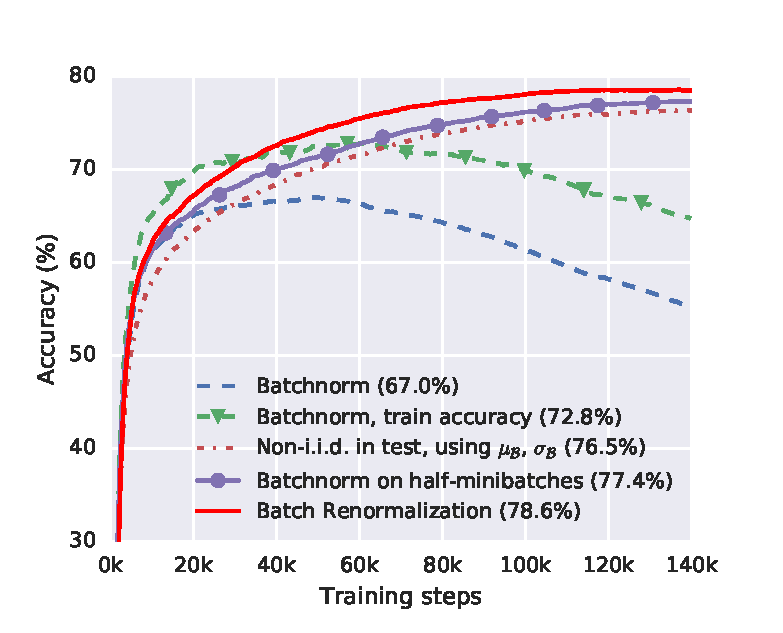
\includegraphics[width=\columnwidth]{biased.eps}
\end{tabular}
    当在 non-i.i.d. minibatch 上训练时所得到的验证准确度,这是通过为 16 个(取自共 1000 个)随机标签中的每一个标签采样 2 张图像得到的。这种分布偏差不仅会导致测试的低准确度,也会导致在训练集上的低准确度,最后还会下降。这表明在这个特定的 minibatch 分布上出现了过拟合,这通过我们的改进得到了证实——当测试 minibatch 也是每个标签包含 2 张图像,并且批规范化在推理过程中使用了 minibatch 统计 µB、σB 时。如果批规范化被分别应用于一个训练 minibatch 的两半,使其中每一半都更 i.i.d.,那么它还会进一步提升。最后,通过使用批再规范化,我们可以仅通过正常的训练和评估就实现如我们在图 1 中的 i.i.d. minibatch 上所得到的同样的验证准确度。
    \caption{\em Validation accuracy when training on non-i.i.d. minibatches, obtained by sampling 2 images for each of 16 (out of total 1000) random labels. This distribution bias results not only in a low test accuracy, but also low accuracy on the training set, with an eventual drop. This indicates overfitting to the particular minibatch distribution, which is confirmed by the improvement when the test minibatches also contain 2 images per label, and batchnorm uses minibatch statistics $\mu_\setB$, $\sigma_\setB$ during inference. It improves further if batchnorm is applied separately to 2 halves of a training minibatch, making each of them more i.i.d. Finally, by using Batch Renorm, we are able to just train and evaluate normally, and achieve the same validation accuracy as we get for i.i.d. minibatches in Fig. \ref{fig-baseline}.
    }
    \label{fig-biased}
\end{figure}

当minibatch中的样本不是独立采样时,批规范化可能表现较差。带依赖的采样可能对于有些任务是必要的,如度量学习。我们可能想要保证具有相同标签的图比那些不同标签的图有更相似的表示,想要学习到这个,我们需要在同一minibatch中发现合理数量的相同标签图相对。
When examples in a minibatch are not sampled independently, batchnorm can
perform rather poorly. However, sampling with dependencies  may be necessary for tasks such as for metric learning \cite{nca,facenet}. We may want to ensure that images with the same label have more similar representations than otherwise, and to learn this we require that a reasonable number of same-label image pairs can be found within the same minibatch.

在这个实验中,每个大小为32的minibatch通过随机抽样的16个标签(总1000)代替,然后对于每个标签随机选择2张图像。批规范化训练的时候,测试精度是比独立同分布样本低,只有$67\%$。惊讶的是,甚至训练精度比独立同分布样本的测试精度要低。事实上,drop的表现跟过拟合是一致的。我们怀疑在实际中会发生,这不直接翻译到单独的图像分类,从而产生训练数据的精度计算下降。为了验证这一点,我们也评估在``训练模式"的模型,例如,使用minibatch统计值$\mu_\setB$, $\sigma_\setB$而不是移动平均$\mu$, $\sigma$,,每个测试minibatch大小为50,使用相同的过程采样出训练minibatch -- 25个标签,每个标签两张图。正如预期的那样,这样表现更好,得到$76.5\%$,尽管准确率仍在基线之下。当然,这种评估方案通常是不可行的,因为我们希望图像表示是确定性的单图像功能。
In this experiment (Figure \ref{fig-biased}), we selected each minibatch of size 32 by randomly sampling 16 labels (out of the total 1000) with replacement, then randomly selecting 2 images for each of those labels.模型学习预测标签的图像在一个集合,其中每个图像具有同一标签的对应物
When training with batchnorm, the test accuracy is much lower than for i.i.d. minibatches, achieving only $67\%$. Surprisingly, even the {\em training} accuracy is much lower ($72.8\%$) than the {\em test} accuracy in the i.i.d. case, and in fact exhibits a drop that is consistent with overfitting. We suspect that this is in fact what happens: the model learns to predict labels for images that come in a set, where each image has a counterpart with the same label. This does not directly translate to classifying images individually, thus producing a drop in the accuracy computed on the training data. To verify this, we also evaluated the model in the ``training mode", i.e. using minibatch statistics $\mu_\setB$, $\sigma_\setB$ instead of moving averages $\mu$, $\sigma$, where each test minibatch had size 50 and was obtained using the same procedure as the training minibatches -- 25 labels, with 2 images per label. As expected, this does much better, achieving $76.5\%$, though still below the baseline accuracy. Of course, this evaluation scenario is usually infeasible, as we want the image representation to be a deterministic function of that image alone.

我们可以将每个minibatch分成一半的大小为16个来改善准确性问题,使每对图像属于同一类的,一张图像被分配到第一半minibatch,另一张图像被分为另一半minibatch。每一半具有更大的独立同分布性质,这就得到了一个更好的测试精度(在140K的步骤$77.4\%$ ),但仍低于基线。这种方法只适用于每个标签的样本数量很小的时候(因为这决定了一个minibatch 需要被分成更小的microbatches)。
We can improve the accuracy for this problem by splitting each minibatch into two halves of size 16 each, so that for every pair of images belonging to the same class, one image is assigned to the first half-minibatch, and the other to the second. Each half is then more i.i.d., and this achieves a much better test accuracy ($77.4\%$ at 140k steps), but still below the baseline. This method is only applicable when the number of examples per label is small (since this determines the number of microbatches that a minibatch needs to be split into).

对于批再规范化,我们简单的以大小为32的minibatch训练模型,模型在120k 步之后获得同样的测试精度$78.5\%$作为独立同分布的等效模型,而批规范化只有$67\%$的精度。通过用批再规范化取代批规范化,我们保证推断模型可以有效的区分单张图像。这已经完全消除了过度拟合的模型与偏见的标签分布图像集的影响。
With Batch Renorm, we simply trained the model with minibatch size of 32. The model achieved the same test accuracy ($78.5\%$ at 120k steps) as the equivalent model on i.i.d. minibatches, vs. $67\%$ obtained with batchnorm. By replacing batchnorm with Batch Renorm, we ensured that the inference model can effectively classify individual images. This has completely eliminated the effect of overfitting the model to image sets with a biased label distribution.


\section{Conclusions}
我们指出,批规范化虽然有效,但不适合小minibatch或者非独立同分布训练样本。我们假设这些缺点是由于在实际中,模型的激活反过来作为其他层的输入,梯度计算训练过程跟推断过程不同。我们提出了批再规范化,替代批规范化模型的输出计算在训练和推断阶段都只仅仅依赖于个别样本而不是整个的minibatch。

We have demonstrated that Batch Normalization, while effective, is not well suited to small or non-i.i.d. training minibatches. We hypothesized that these drawbacks are due to the fact that the activations in the model, which are in turn used by other layers as inputs, are computed differently during training than during inference. We address this with Batch Renormalization, which replaces batchnorm and ensures that the outputs computed by the model are dependent only on the individual examples and not the entire minibatch, during both training and inference.

批再规范化对批规范化进行了单维修正,来保证训练网络和推断网络的激活匹配。这种修正的期望是恒同变换;修正参数是从minibatch中计算出来的,但是在优化过程中被当做一个常数。在批规范化中,我们在训练完成之后才进行计算将在推断过程使用的均值和方差,而批再规范化的好处在在训练过程中就使用这些参数。
批再规范化与批规范化一样易于实现,训练和推断速度也没有差别,但是却明显的改善了模型在小minibatch和非独立同分布minibatch上的训练效果。
我们的方法需要引入额外的超参数:移动平均的更新率$\Delta$,修正参数的取值上限$\dmax$, $\rmax$。对于这些超参数的影响更深入的研究是未来工作的一部分。

Batch Renormalization extends batchnorm with a per-dimension correction to ensure that the activations match between the training and inference networks. This correction is identity in expectation; its parameters are computed from the minibatch but are treated as constant by the optimizer. Unlike batchnorm, where the means and variances used during inference do not need to be computed until the training has completed, Batch Renormalization benefits from having these statistics directly participate in the training. Batch Renormalization is as easy to implement as batchnorm itself, runs at the same speed during both training and inference, and significantly improves training on small or non-i.i.d. minibatches. Our method does have extra hyperparameters: the update rate $\Delta$ for the moving averages, and the schedules for correction limits $\dmax$, $\rmax$. A more extensive investigation of the effect of these is a part of future work.

批再规范化可以改善任何正常使用批规范化模型的性能,包括残差网络\cite{resnet}。另一个应用是在生成式对抗网络中\cite{gan},批规范化引入的非确定性被发现是个问题,而批再规范化有可能会为这个问题提供一个解决方案。

Batch Renormalization offers a promise of improving the performance of any model that would normally use batchnorm. This includes Residual Networks \cite{resnet}. Another application is Generative Adversarial Networks \cite{gan}, where the non-determinism introduced by batchnorm has been found to be an issue, and Batch Renorm may provide a solution.

最后,批再规范化可能对那些应用批规范化困难的应用有效,例如递归网络。在这些情况种,批规范化要求每个时间戳独立正则化(难以做到)。而批再规范化令使用同一个移动平均来规范化所有时间戳,然后再使用所有时间戳来更新那些均值这种做法成为可能。但这仍然是未来值得深入探索的一个领域。

Finally, Batch Renormalization may benefit applications where applying batch normalization has been difficult -- such as recurrent networks. There, batchnorm would require each timestep to be normalized independently, but Batch Renormalization may make it possible to use the same running averages to normalize all timesteps, and then update those averages using all timesteps. This remains one of the areas that warrants further exploration.
